% This is "sig-alternate.tex" V2.0 May 2012
% This file should be compiled with V2.5 of "sig-alternate.cls" May 2012
%
% This example file demonstrates the use of the 'sig-alternate.cls'
% V2.5 LaTeX2e document class file. It is for those submitting
% articles to ACM Conference Proceedings WHO DO NOT WISH TO
% STRICTLY ADHERE TO THE SIGS (PUBS-BOARD-ENDORSED) STYLE.
% The 'sig-alternate.cls' file will produce a similar-looking,
% albeit, 'tighter' paper resulting in, invariably, fewer pages.
%
% ----------------------------------------------------------------------------------------------------------------
% This .tex file (and associated .cls V2.5) produces:
%       1) The Permission Statement
%       2) The Conference (location) Info information
%       3) The Copyright Line with ACM data
%       4) NO page numbers
%
% as against the acm_proc_article-sp.cls file which
% DOES NOT produce 1) thru' 3) above.
%
% Using 'sig-alternate.cls' you have control, however, from within
% the source .tex file, over both the CopyrightYear
% (defaulted to 200X) and the ACM Copyright Data
% (defaulted to X-XXXXX-XX-X/XX/XX).
% e.g.
% \CopyrightYear{2007} will cause 2007 to appear in the copyright line.
% \crdata{0-12345-67-8/90/12} will cause 0-12345-67-8/90/12 to appear in the copyright line.
%
% ---------------------------------------------------------------------------------------------------------------
% This .tex source is an example which *does* use
% the .bib file (from which the .bbl file % is produced).
% REMEMBER HOWEVER: After having produced the .bbl file,
% and prior to final submission, you *NEED* to 'insert'
% your .bbl file into your source .tex file so as to provide
% ONE 'self-contained' source file.
%
% ================= IF YOU HAVE QUESTIONS =======================
% Questions regarding the SIGS styles, SIGS policies and
% procedures, Conferences etc. should be sent to
% Adrienne Griscti (griscti@acm.org)
%
% Technical questions _only_ to
% Gerald Murray (murray@hq.acm.org)
% ===============================================================
%
% For tracking purposes - this is V2.0 - May 2012

\documentclass[conference]{IEEEtran}

%preambles
\usepackage{alltt                                    % I like these
          , multirow
          , booktabs
          , listings
          , graphicx
          ,float
	,cite
          ,verbatim
         ,mathtools
	,url
	,amsmath
}
\usepackage[table]{xcolor}
\usepackage[numbers]{natbib}     % this is a better citation system
\usepackage{syntax}
\usepackage{algorithmic, algorithm}
\usepackage{enumitem}
\usepackage{threeparttable}
\usepackage{framed}

\usepackage{expl3}
\ExplSyntaxOn
\newcommand\latinabbrev[1]{
  \peek_meaning:NTF . {% Same as \@ifnextchar
    #1\@}%
  { \peek_catcode:NTF a {% Check whether next char has same catcode as \'a, i.e., is a letter
      #1., \@ }%
    {#1., \@}}}
\ExplSyntaxOff

%switch case statement
\newcommand{\SWITCH}[1]{\STATE \textbf{switch} (#1)}
\newcommand{\ENDSWITCH}{\STATE \textbf{end switch}}
\newcommand{\CASE}[1]{\STATE \textbf{case} #1\textbf{:} \begin{ALC@g}}
\newcommand{\ENDCASE}{\end{ALC@g}}
\newcommand{\CASELINE}[1]{\STATE \textbf{case} #1\textbf{:} }
\newcommand{\DEFAULT}{\STATE \textbf{default:} \begin{ALC@g}}
\newcommand{\ENDDEFAULT}{\end{ALC@g}}
\newcommand{\DEFAULTLINE}[1]{\STATE \textbf{default:} }
%switch case statement
\let\footnotesize\scriptsize


\newsavebox{\supbox}% Superscript box
\newcommand{\bsup}{\begin{lrbox}{\supbox}$\tt\scriptstyle}% Superscript begin
\newcommand{\esup}{$\end{lrbox}{}^{\usebox{\supbox}}}% Superscript end
\def\eg{\latinabbrev{e.g}}
\def\ie{\latinabbrev{i.e}}

%\dimen0=\ht\@acmtitlebox
%\ifdim\dimen0<0.0pt\relax\vskip-\dimen0\fi}

\renewcommand{\labelenumi}{(\alph{enumi})}

\definecolor{lightpurple}{rgb}{0.8,0.8,1}
\definecolor{codebg}{RGB}{255,255,255}
\definecolor{commentcolor}{RGB}{11,140,11}
%listing settings
\lstset{ 
    language=java, % choose the language of the code
    basicstyle=\fontfamily{pcr}\selectfont\scriptsize\color{black},
    keywordstyle=\color{blue}\bfseries, % style for keywords
   commentstyle=\color{commentcolor},
    numbers=none, % where to put the line-numbers
    numberstyle=\tiny, % the size of the fonts that are used for the line-numbers     
    backgroundcolor=\color{codebg},
    showspaces=false, % show spaces adding particular underscores
    showstringspaces=false, % underline spaces within strings
    showtabs=false, % show tabs within strings adding particular underscores
    frame=single, % adds a frame around the code
    tabsize=2, % sets default tabsize to 2 spaces
    rulesepcolor=\color{gray},
    %rulecolor=\color{black},
    captionpos=b, % sets the caption-position to bottom
    breaklines=true, % sets automatic line breaking
    breakatwhitespace=false, 
}

%\newcommand{\footremember}[2]{%
%   \footnote{#2}
%    \newcounter{#1}
%    \setcounter{#1}{\value{footnote}}%
%}
%\newcommand{\footrecall}[1]{%
%    \footnotemark[\value{#1}]%
%} 


\begin{document}
%
% --- Author Metadata here ---
%\conferenceinfo{WeTSOM}{'2014, Hyderabad India}
%\CopyrightYear{2007} % Allows default copyright year (20XX) to be over-ridden - IF NEED BE.
%\crdata{0-12345-67-8/90/01}  % Allows default copyright data (0-89791-88-6/97/05) to be over-ridden - IF NEED BE.
% --- End of Author Metadata ---

\title{Code Quality in the Eyes of Crowd and in Terms of Metrics: A Comparative Study using Stack Overflow}
%
% You need the command \numberofauthors to handle the 'placement
% and alignment' of the authors beneath the title.
%
% For aesthetic reasons, we recommend 'three authors at a time'
% i.e. three 'name/affiliation blocks' be placed beneath the title.
%
% NOTE: You are NOT restricted in how many 'rows' of
% "name/affiliations" may appear. We just ask that you restrict
% the number of 'columns' to three.
%
% Because of the available 'opening page real-estate'
% we ask you to refrain from putting more than six authors
% (two rows with three columns) beneath the article title.
% More than six makes the first-page appear very cluttered indeed.
%
% Use the \alignauthor commands to handle the names
% and affiliations for an 'aesthetic maximum' of six authors.
% Add names, affiliations, addresses for
% the seventh etc. author(s) as the argument for the
% \additionalauthors command.
% These 'additional authors' will be output/set for you
% without further effort on your part as the last section in
% the body of your article BEFORE References or any Appendices.

\author{\IEEEauthorblockN{Mohammad Masudur Rahman  ~~~ Chanchal K. Roy ~~~$^1$Iman Keivanloo}
\IEEEauthorblockA{University of Saskatchewan, $^1$Queen's University, Canada\\
\{masud.rahman, chanchal.roy\}@usask.ca, $^1$iman.keivanloo@queensu.ca}
}

%\numberofauthors{3} %  in this sample file, there are a *total*
% of EIGHT authors. SIX appear on the 'first-page' (for formatting
% reasons) and the remaining two appear in the \additionalauthors section.
%
%\author{
% You can go ahead and credit any number of authors here,
% e.g. one 'row of three' or two rows (consisting of one row of three
% and a second row of one, two or three).
%
% The command \alignauthor (no curly braces needed) should
% precede each author name, affiliation/snail-mail address and
% e-mail address. Additionally, tag each line of
% affiliation/address with \affaddr, and tag the
% e-mail address with \email.
%
% 1st. author
%\alignauthor
%\begin{tabular}[t]{@{}c@{}}
%Mohammad Masudur Rahman~~~~~ Chanchal K. Roy \\
%       \affaddr{University of Saskatchewan, Canada}\\
%       \email{\{mor543, ckr353\}@mail.usask.ca}
%% 2nd. author
%\end{tabular}
%% 3rd. author
%\alignauthor
%Iman Keivanloo\\
%       \affaddr{Queen's University, Canada}\\
%       \email{iman.keivanloo@queensu.ca}
%}

% There's nothing stopping you putting the seventh, eighth, etc.
% author on the opening page (as the 'third row') but we ask,
% for aesthetic reasons that you place these 'additional authors'
% in the \additional authors block, viz.
%\additionalauthors{Additional authors: John Smith (The Th{\o}rv{\"a}ld Group,
%email: {\texttt{jsmith@affiliation.org}}) and Julius P.~Kumquat
%(The Kumquat Consortium, email: {\texttt{jpkumquat@consortium.net}}).}
%\date{30 July 1999}
% Just remember to make sure that the TOTAL number of authors
% is the number that will appear on the first page PLUS the
% number that will appear in the \additionalauthors section.
%StackOverflow, a popular programming Q \& A site, often contains working code examples that solve particular programming problems, as a part of the answers against the posted questions. Studies show that the community is highly interested of those code examples, and the examples contribute greatly to the promotion and demotion of the answers. 
\maketitle

\begin{abstract}
In StackOverflow, code examples are generally analyzed and subjectively evaluated by a large crowd of technical users. Given the growing interest of those examples to the community and their undeniable role in answers, we are motivated to study whether the subjective quality of those examples as perceived by StackOverflow actually matches with their metric-based quality. This is an important piece of information for the developers willing to reuse such examples. In this paper, we propose and evaluate a metric-based quality model for StackOverflow code examples by conducting an exploratory study where we analyze 160 code examples from 80 programming problems. Our quality model agrees with StackOverflow for 85.18\% of the test examples in relative quality prediction, which is interesting, and the finding reveals effectiveness and reliability of the subjective evaluation by StackOverflow. 
%While the preliminary findings are promising, they must be evaluated with larger dataset.
\end{abstract}

% A category with the (minimum) three required fields
%\category{H.4}{Information Systems Applications}{Miscellaneous}
%A category including the fourth, optional field follows...
%\category{D.2.8}{Software Engineering}{Metrics}[maintainability measures, reusability measures]
%\terms{Theory, Metrics, Human factors}
%\keywords{Code quality, readability, reusability, maintainability}
\begin{IEEEkeywords}
Objective code quality, readability, maintainability, subjective evaluation
\end{IEEEkeywords}

\IEEEpeerreviewmaketitle



%\vspace{-.2cm}
\section{Introduction}
Studies suggest that software developers spend about 19\% of their development time in searching for relevant code on the web \cite{twostudy}. Stack Overflow, a popular online programming Q \& A site, contains 10 millions questions on various programming topics, and they are used by a large community of 4 million technical users as of April 2014 \cite{sowiki}. In this site, users promote a question or an answer through up-voting when they find it useful or informative, and down-voting a post when they find its content erroneous or off-topic. The difference between up-votes and down-votes is considered as the \emph{score} for the post. 

During development and maintenance of a software product, software developers deal with different programming problems or challenges, and they frequently look into the programming issues posted on StackOverflow. The answers posted on the site often contain working code examples (\ie\ code fragments) that solve particular programming problems or accomplish certain programming tasks. The developers find such examples helpful and reusable, and they also frequently apply them in their daily problem solving or learning activities. The posted code examples are generally viewed and subjectively evaluated (\ie\ voting) by a large crowd of technical users. However, the objective quality of those examples is not often taken into consideration by the developers during reuse. Reusing or consulting with such code examples can be a threat if the promoted (\ie\ up-voted) examples by the crowd maintain low quality in terms of objective code metrics.

\citet{nasehi} study the characteristics of the accepted answers of 163 programming questions from StackOverflow, and argue that  the accepted answers are most likely to contain efficient and concise code examples accompanied by comprehensive textual description. Their study also reveals that the discouraged (\ie\ extensively down-voted) answers from StackOverflow either do not contain code examples or miss the explanation about the code. \citet{nier} study which type of questions are answered correctly for most of the time, and suggest that the answers of the \emph{code-review questions} (\ie\ containing code examples) have the maximum acceptance rate of 92\%.
While these studies demonstrate the importance or the influence of StackOverflow code examples, the quality of those examples is not yet studied from metric-based point of view.

\begin{figure*}[!t]
\centering
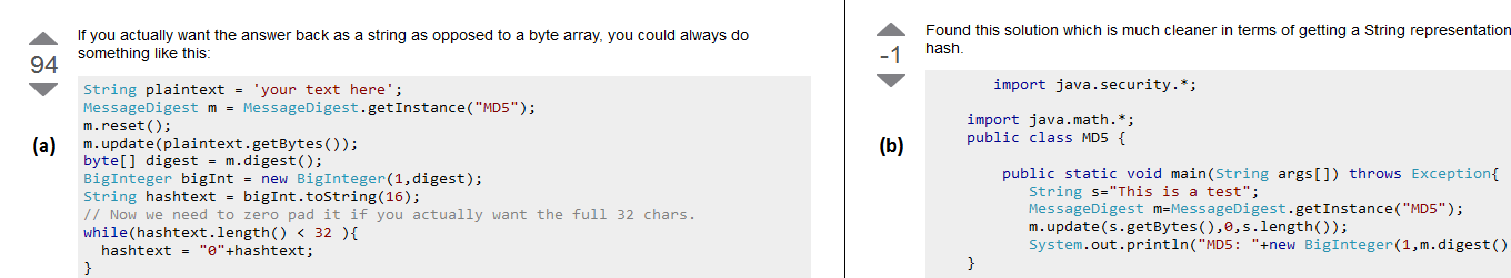
\includegraphics[width=6.8in ]{whole23}
\caption{(a) Promoted code example, (b) Discouraged code example}
\vspace{-.2cm}
%\label{fig_sim}
\label{fig:example}
\end{figure*}

%Given that the code examples either in question posts or answer posts are of great interest to the community \cite{nasehi, nier}, it is reasonable to conjecture that  StackOverflow users often consult with them or more precisely reuse them in their everyday programming activities. Basically, this increased interest of the community on code examples provides us the motivation for their classification or reevaluation. As \citeauthor{nasehi} suggest, code examples arguably play a major role behind the \emph{acceptance} or \emph{rejection} of a programming answer by the community, 
%
%they also can be categorized as \emph{promoted} (\ie\ extracted from promoted answer) or \emph{discouraged} (\ie\ extracted from discouraged answer) ones analogously based on the \emph{scores} of their corresponding posts. However, it is essential to check the code level quality of those code examples given that millions of StackOverflow users are using them for their problem solving. 

%However, the vote score-based classification of the code examples suffers from several limitations. First, the votes can be considered as the quantification of the evaluation by the community users, which is based on their subjective viewpoints. The viewpoints may vary based on the expertise level, interests or demographics of the users, and therefore, the \emph{vote score} may not reflect a representative measure for the quality of the code example. Second, evaluations (\ie\ votes) both from expert and novice users are considered with equal importance which makes the vote score unreliable. Third, vote score of a code example (\ie\ answer post) can be influenced by its age and exposure to the community. That means, a recently introduced good code example may have the vote score equal to that of a moderate quality example introduced long ago; however, the classification does not consider those factors and treats both code examples  as of equal merit. Thus, it is pretty evident that score-based annotation of the code examples is affected by certain unattended factors, and
A number of existing studies focus on code level metrics for checking readability \cite{readability}, reusability \cite{reusability} or overall quality \cite{lochmann, survey} of the software code. \citet{reusability} studies reusability of 33 open source projects based on code level metrics such as understandability, low complexity and modularity, and proposes 
a reusability model with different heuristic weights (\ie\ importance) for different metrics. \citet{subjective} conduct an empirical study to determine correlation between subjective evaluation and metric-based evaluation of software quality (w.r.t. code smells), and suggest that no evaluation alone is completely reliable. However, to date, no studies focus on the metric-based quality analysis of the StackOverflow code examples. In this research, we are interested to check whether the perceived quality of the code examples based on code level and associated metrics complies with StackOverflow votes for the corresponding examples. More specifically, we attempt to find out whether the promoted code example (\eg\ Fig. \ref{fig:example}-(a)) is actually preferable to the discouraged one (\eg\ Fig. \ref{fig:example}-(b)) for a programming problem in terms of different objective quality metrics. We formulate the following research question:
\begin{framed}
\noindent
\textbf{RQ$_1$}: Is the metric-based quality of a discouraged code example worse than that of a promoted code example?
\textbf{RQ$_2$}: Can meta data about code examples separate promoted code examples from the discouraged ones?

\end{framed}
%\vspace{-.15cm}
%\begin{itemize}
%\setlength{\topsep}{0pt}
%\item RQ1: Is the code level quality of a discouraged code example worse than that of a promoted code example?
%\item RQ2: Why does not the metric-based classification of the code examples completely agree with vote score-based classification by StackOverflow?
%\end{itemize}
%\vspace{-.15cm}
We conduct an exploratory study using 160 highly promoted and highly discouraged code examples (\ie\ code fragments) from 80 programming problems posted on StackOverflow. We apply five code level metrics-- \emph{readability}, \emph{strength}, \emph{concern}, \emph{documentation} and \emph{methodexist} and two associated metrics-- \emph{authorscore} and \emph{editorscore}, and develop a objective quality model to perceive the quality of those code examples.  Our model agrees with StackOverflow for 85.18\% of the test examples in \emph{relative quality prediction}, which is promising, and it reveals the effectiveness and reliability of the subjective evaluation by StackOverflow. We also investigate the examples for which the model does not agree with StackOverflow on quality analysis, and finally answer the research question.
%The rest of the paper is organized as follows -- Section \ref{sec:theory}  focuses on our adopted methodology and code quality metrics, Section \ref{sec:experiment} discusses the conducted experiments and findings, and finally Section \ref{sec:conclusion} concludes the paper with future works.
\begin{figure}[!t]
\centering
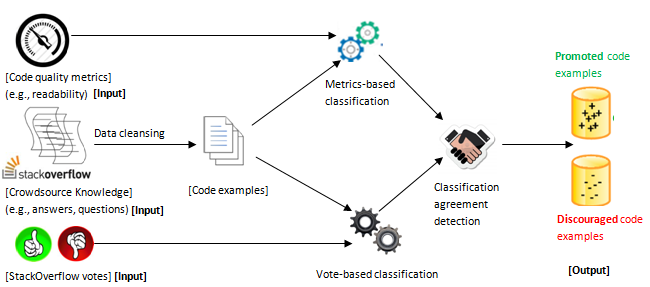
\includegraphics[width=3.1in]{sysdiag}
\caption{Schematic diagram of the conducted study}
\vspace{-.2cm}
\label{fig:sysdiag}
\end{figure}
\vspace{-.2cm}
\section{Methodology}
\label{sec:theory}
Fig. \ref{fig:sysdiag} shows the schematic diagram of our conducted study.
%our approach for objective quality analysis of StackOverflow code examples. 
In this section, we discuss the detailed design of the study, our proposed metrics and proposed model for objective quality analysis of StackOverflow code examples.
\subsection{Data Collection}
We use StackExchange Data API \cite{api} (\ie\ provides access to the data of several StackExchange sites), and collect 80 programming questions along with their answers from StackOverflow which are related to \emph{android platform} and \emph{android applications}.
It should be noted that each of those questions has more than \emph{ten answers} that contain \emph{code examples}. The idea is to collect such questions which are both widely discussed and related to coding. 
We choose three top-ranked and three lowest-ranked answers based on StackOverflow votes for each of those questions. We then extract code examples from the raw HTML of those StackOverflow answers, and manually analyze them.
We look for trivial examples such as \emph{novice's examples} (\ie\ intended for novice users), \emph{abstract examples} (\ie\ too generic) or \emph{small examples} (\ie\ contains less than three lines of code), and discard them in order to develop a list of qualified examples. 
Finally, as discussed in Section \ref{sec:voteclass} below, we select two code examples out of the remaining examples for each question, and one of them is from highly promoted (\ie\ up-voted) answer and the other is from highly discouraged (\ie\ down-voted) answer.

%We collect the latest data dump\cite{dump} provided under creative commons, and extract 75 programming questions and their corresponding answers from it. It should be noted that each of those questions has \emph{more than ten answers that contain code examples}. The idea is to select questions which are widely discussed and coding related. We extract the code examples from the raw HTML of StackOverflow answers, and manually analyze those examples. We find that most of them are not directly compilable (\ie\ necessary to determine a few metrics), and we perform simple tweaking (\eg\ adding import statements or semicolons, declaring undeclared variables and so on) on the examples to make them compilable. However, we also find some code examples are too trivial or they cannot be compiled at all with simple tweaking, which are discarded. Finally, we select 55 programming questions and 110 promoted and discouraged code examples posted in their answers for the study. As discussed in Section \ref{sec:voteclass} below, we select two code examples out of all examples for each question, and one of them is highly promoted (\eg\ up-voted) and the other is highly discouraged (\eg\ down-voted).
\vspace{-.1cm}
\subsection{Vote Based Classification}\label{sec:voteclass}
In StackOverflow, the technical merit or quality of a programming answer is recognized in terms of votes \cite{nasehi}, and code examples are generally posted as a part of those answers. Existing studies \cite{nasehi, nier} report and explain the undeniable role of code examples in the promotion or demotion of the posted answers. Thus the votes cast by thousands of technical users of StackOverflow for those answers can also be considered to approximate the subjective quality of the code examples contained by those answers. Given that the subjective perception of quality may vary, we choose the code examples of two extreme quality perceptions-- highly promoted and highly discouraged. We examine the \emph{scores} (\ie\ difference between up-votes and down-votes) 
achieved to date (\ie\ November 01, 2014) by different answers for each of the 80 programming questions. We then choose the corresponding code examples from the highly promoted (\ie\ up-voted) and the highly discouraged (\ie\ down-voted) answers for each question, and classify them as \emph{highly promoted} and \emph{highly discouraged} code examples respectively.
%of the code examples, and calculate \emph{vote score per day} for each of them. Then, based on the scores gained per day, we choose \emph{a highly promoted} (\eg\ highest scores gained per day) and \emph{a highly discouraged} (\eg\ lowest scores gained per day) code examples for each of 55 questions. 
%We also manually analyze each code example for possible false positives, and to perceive the difference of their relative quality .
%The idea is to determine whether the subjective evaluation of the code examples agrees with the metric-based evaluation. We also manually analyze each code example for possible false positives, and to perceive their relative quality difference.
%Generally StackOverflow code examples are small-sized code fragments; in our case, we find them less than 15 lines on average. The 
\vspace{-.1cm}
\subsection{Objective Quality Metrics}
\label{sec:metrics}
StackOverflow code examples are generally posted either as complete methods or code segments containing a few lines, and the entire \emph{class-structure} is often unlikely. Therefore, most of the available code quality metrics such as \emph{object-oriented complexity} metrics are not applicable for those examples. In this section, we discuss five code related metrics and two associated metrics used for the study. 

\textbf{Readability (R)}: Readability of software code refers to a human judgement of how easy the code is to understand \cite{readability}. Reading (\ie\ understanding) code is one of the most time-consuming components of all software maintenance activities, and thus, readability is directly related to software maintainability. 
%Study suggests that readability also greatly contributes to reusability and portability of the code \cite{readability}. Thus, readability is an established code quality metric, and 
The baseline idea is-- the more readable or understandable the code is, the easier it is to reuse and maintain in the long run. \citet{readability} propose a code readability model trained on human perception of readability or understandability. The model uses different textual source features (\eg\ length of identifiers, number of comments, line length) that are likely to affect the humans' perception of readability, and predicts a \emph{readability score} on the scale from zero to one, inclusive, with one describing that the source code is highly readable. We use the readily available library\cite{readlib} by \citet{readability} for calculating the \emph{readability metric} of the code examples.
 
\textbf{Author Rank (AR) \& Editor Rank (ER)}: As existing studies \cite{specmining} suggest, we believe that the expertise of the author or an editor of a code example is likely to influence its quality. 
StackOverflow provides different incentives to the users who actively contribute to the body of knowledge by asking important questions, posting helpful answers or adding informative comments. One of those incentives is \emph{Reputation} (\ie\ an estimation of overall contribution to the site) which can be often considered as an approximation of one's expertise. 
%\citet{specmining} s \emph{author expertise} as an influencer of code quality for specification mining, and in our study, we also use it with a focus on reusability of the code examples. 
In order to determine \emph{author rank} and \emph{editor rank} of a code example, we collect the \emph{reputation scores} of the author and the last editor of that example. We then normalize these scores against the \emph{maximum user reputation} from StackOverflow, and provide both metrics on the scale from zero to one, where zero denotes the least expertise and vice versa.
%consider the \emph{Reputation} of the corresponding author and the \emph{Maximum Reputation} among all authors of StackOverflow. Then we provide a normalized estimate on the scale from zero to one, where zero denotes the least experience.

\textbf{Strength (S) and Concern (W)}: \citet{subjective} conduct an empirical study on software evolvability by employing subjective and metric-based identification of code smells.
They analyze agreement level between the two evaluations, and argue that neither technique alone is enough to detect all smells. 
Similarly, we can conjecture that code level metrics are not sufficient enough to discover all types of defects, inefficiencies or possible scopes for improvement in the code examples. StackOverflow facilitates to include the subjective evaluations for each code example in the form of comments which often contain invaluable and insightful analysis about its code level quality. While one can argue that the comments are merely based on subjective viewpoints, we note that they also contain objective observations which can be considered to derive metrics describing the soundness of the code example. We leverage the objective observations to identify the strengths and weaknesses of the code example. Basically, we analyze all the comments about a code example against the code and count their numbers discussing about positive aspects (\ie\ strength) and negative aspects (\ie\ weakness) of the code. Then we normalize the \emph{strength} and \emph{weakness} measures using \emph{maximum comment count} among the code examples of the \emph{same question} as follows.
\begin{equation}
\vspace{-.1cm}
S_{i}=\frac{S_{i, count}}{max(TC_{i})},~~~ W_{i}=\frac{W_{i, count}}{max(TC_{i})}
\vspace{-.1cm}
\end{equation}
Here, $S_{i, count}, W_{i, count}$ and $TC_{i}$ denote the positive comments count, negative comments count and total comments count of a code example respectively. Both the \emph{strength} and \emph{weakness} metrics provide a normalized score on the scale from zero to one, where zero represents the least measure of each metric. 

%Deviation from standard coding practices can be considered as an important measure to estimate the code quality of the code examples.
\textbf{Rule Violation (RV)}: Traditional metric-based quality evaluation is dominated by code analysis tools, and they try to analyze the code against a certain set of \emph{ recommended rules}. Most of the tools concentrate on  particular aspects of code. For example, \emph{CheckStyle} focuses on conventions, \emph{PMD} on bad practices and \emph{FindBugs} focuses on potential bugs or threats. Thus, rules and standards of one tool may vary from another, and the tools are no way competitive rather complementary. Given the facts about the tools, using any single one may not serve our purpose of detecting rule violations, and thus we use \emph{sonarQube}\footnote{http://www.sonarqube.org/} which combines the rules and standards of \emph{PMD, FindBugs, CheckStyles} and so on. We collect three types of violations -- critical, major and minor, in the code examples and determine \emph{violations per source line} for each of them. \citet{lochmann} propose a rule-based quality model for the comprehensive quality assessment of a complete software project using the rules extracted from static code analysis tools. However, given the coding structure and size of StackOverflow code examples, we hypothesize that \emph{violation per source line} is an important and credible metric to estimate the relative quality of the code examples. In order to preserve uniformity with other metrics, we normalize \emph{violation per source line} for each code example.
\vspace{-.1cm}
\subsection{Metric-Based Quality Model}
We consider readability, author's expertise, adherence to the best coding practices, identified issues and threats in the code examples to estimate the quality of the examples with the focus on their reusability. We randomly select 50 code examples from 25 programming questions in the dataset, analyze their quality, and manually label them either as \emph{promoted} or \emph{discouraged}. Then we use those labeled examples along with their computed metrics (\ie\ Section \ref{sec:metrics}), and use logistic regression-based classifier from \emph{Weka} to determine the relative predictive power of the proposed metrics. It should be noted that we use Odd Ratio \cite{specmining} of each metric, which is a logarithmic transformation of the metric coefficient in the regression equation of the classifier, and tune them under controlled iterations to determine the predictive power (\ie\ importance) of the metric. Since, we are interested in determining the relative quality (\ie\ without a threshold) of two code examples of the same question, we ignore the intercept of the equation, and develop the following quality model. 
% Finally, we develop the following quality model to perform the relative quality analysis among the code examples, where the coefficients are the predictive power (\ie\ importance) of corresponding metrics.
\begin{equation}\label{eq:model}
\vspace{-.1cm}
\begin{split}
Q_{i}=3.0043\times R_{i}+4.3067\times AR_{i}
+8.04884\times S_{i}\\+0.5078\times W_{i}+0.5812\times RV_{i}
\end{split}
\vspace{-.1cm}
\end{equation}
In the model, we find \emph{readability}, \emph{author rank}, and \emph{strength} as the most dominating features (\ie\ metrics), whereas \emph{weakness} and \emph{rule violation} as the least influencing ones. It should be noted that the first three of the metrics are positive factors for software code quality (\ie\ improves quality) and the rest two are negative factors (\ie\ degrades quality). Since, we are interested in the relative quality assessment of the code examples, we use the logarithmic transformation that provides different Odd Ratios (\ie\ weights) of the metrics within the same range (\ie\ greater than zero) and makes the quality estimates more comprehensive.

\vspace{-.1cm}
\section{Results and Discussions}
\label{sec:experiment}
In our experiment, we use the proposed quality model to estimate the quality of 110 code examples against 55 programming questions (dataset can be found online\footnote{www.usask.ca/$\sim$masud.rahman/ss/expdata}). It should be noted that we use the quality estimates to perform the comparative analysis among the two code examples of the same question. The idea is to determine whether a code example promoted by StackOverflow is actually of better code quality than the one which is discouraged by it from metric-based point of view. Table \ref{table:result} shows the results of our preliminary experiments using Equation \eqref{eq:model}, where the metric-based relative quality of the code examples agrees with that of StackOverflow at best for 43 (78.18\%)  out of 55 questions. It also shows how different component quality metrics can influence the estimated overall quality of the code examples, and the empirical findings show that \emph{readability}(R), \emph{author rank}(AR) and \emph{strength}(S) are the most effective metrics for relative quality analysis when they are considered in combination. We note that \emph{weakness} and \emph{rule violation} metrics have a little or no influence to the proposed model, which refutes our initial assumption.
\begin{table}
\centering
\caption{Experimental Results}\label{table:result}
\resizebox{2.5in}{!}{%
\begin{threeparttable}
\begin{tabular}{l|c|c|c}
\hline
\textbf{Metrics} & \textbf{APC}\tnote{1} & \textbf{A}\tnote{2} & \textbf{D}\tnote{3}\\
\hline
%\{R\} & 25(55) & 45.45\% & 54.55\%\\
%\hline
%\{AR\} & 32(55) & 58.18\% & 41.82\%\\
%\hline
%\{S\} & 30(55) & 54.55\% & 45.45\%\\
%\hline
%\{W\} & 22(55) & 40.00\% & 60.00\%\\
%\hline
%\{RV\} & 24(55) & 43.64\% & 56.36\%\\
%\hline
\{R, AR\} & 30(55) & 54.55\% & 45.45\%\\
\hline
\{R, S\} & 39(55) & 70.91\% & 29.09\%\\
\hline
\{R, W\} & 29(55) & 52.72\% & 47.28\%\\
\hline
\{R, AR, S\} & \textbf{42(55)} & \textbf{76.36\%} & \textbf{23.64\%} \\
\hline
\{R, S, W\} & 41(55) & 74.54\% & 25.45\% \\
\hline
\{R, AR, S, W\} & \textbf{43(55)} & \textbf{78.18\%} & \textbf{21.82\%} \\
\hline
\{R, S, W, RV\} &  41(55) & 74.54\% & 25.45\% \\
\hline
\{R, AR, S, W, RV\} & \textbf{43(55)} & \textbf{78.18\%} & \textbf{21.82\%} \\
\hline
\end{tabular}
%\begin{tablenotes}
%\item [1] No. of example pairs for which relative quality evaluation matches with that of StackOverflow
%\item [2] \% of agreement, \item [3] \% of disagreement
 $^1$No. of example pairs for which relative quality evaluation matches with that of StackOverflow, \\
$^2$ \% of agreement, $^3$ \% of disagreement
 %\end{tablenotes}
\end{threeparttable}

%\vspace{-.2cm}
}
\vspace{-.5cm}
\end{table}

\begin{table}
\centering
\caption{Metrics Correlation}\label{table:correlation}
\resizebox{3in}{!}{%
\begin{threeparttable}
\begin{tabular}{l|c|c||l|c|c}
\hline
\textbf{Metrics} & \textbf{CR}\tnote{1} & \textbf{P}\tnote{2} & \textbf{Metrics} & \textbf{CR}& \textbf{P}\\
\hline
R, AR & -0.1767 & 0.0647 & AR, S & 0.1164 & 0.2258 \\
\hline
R, S & -0.0916 & 0.3412 & AR, W & 0.1045 & 0.2772 \\
\hline
R, W & -0.0512 & 0.5954 & S, W & -0.2321 & 0.0147 \\
\hline
\end{tabular}
%\begin{tablenotes}
%\item [1] No. of example pairs for which relative quality evaluation matches with that of StackOverflow
%\item [2] \% of agreement, \item [3] \% of disagreement
$^1$Correlation, $^2$p-value
 %\end{tablenotes}
\end{threeparttable}

%\vspace{-.2cm}
}
\vspace{-.5cm}
\end{table}






% that the answer is \emph{yes} for about 78\% of the time.
\emph{RQ: Is the code level quality of a discouraged code example worse than that of a promoted code example?} Our preliminary results (Table \ref{table:result}) indicate that the code quality of discouraged code examples is worse than that of promoted code examples in 78\% of the examples. Based on the subjective evaluation (\eg\ score per day) by StackOverflow, we estimated the relative quality of the two code examples against each of our selected questions, and determined the \emph{promoted} and the \emph{discouraged} ones. In order to determine their code level quality, we collected the target quality metrics (Section \ref{sec:metrics}) of each code example, and applied them to the proposed quality model. The model provides an estimate about the quality of each example, and we used those estimates to determine the relative code quality of the two code examples against a question. Then we compared the metric-based relative quality against the corresponding relative quality obtained from subjective evaluation. The result shows that the discouraged code examples are of inferior quality in terms of code metrics to the promoted ones for 43 (78.18\%) test cases out of 55 cases.

%\emph{RQ2: Why does not the metric-based classification of the code examples completely agree with vote score-based classification by StackOverflow?} 
According to our experiment,  the two classifications agree mostly, about 78\%; however, the complete agreement may not be possible. We investigated the 12 cases (24 code examples and their metrics) for which our quality model does not match with StackOverflow, and found a few issues or scenarios. First, most of them do not contain comments given that metrics (\eg\ strength and weakness) from the comments play major parts in our model, and the model does not perform well for those cases (\ie\ 9 cases). Second, our model does not use any threshold to describe a code example either as promoted or discouraged, rather it uses relative quality analysis which may not be effective all the time. For example, if there is a little difference in the quality estimate of two code examples, the model still determines the promoted and discouraged ones; however, both of them should be considered either as promoted or discouraged in practical. We found one such case in the experiment. Third, StackOverflow contains some code examples, which are highly simplified with little technical merit, and are often intended for preliminary learning, and they are also highly voted. Our model does not perform well in that case (\ie\ 3 cases). 
%Fourth, we also found some cases where \emph{vote score} does not necessarily represent the evaluation of the contained code examples or code examples do not play major part in answering the question, and our model does not perform well in those cases.

Given that \emph{code quality} of the software code is a multifaceted term \cite{survey}, we focus on the quality analysis to determine the \emph{reusability} of a code example. \emph{Readability}, \emph{strength}, \emph{weakness} and \emph{rule violation} metrics are greatly related to comprehensibility, efficiency, security, maintainability and other attributes (\ie\ quality) of the software code that stimulate its reuse \cite{readability}. In our experiment, we found \emph{strength}(\eg\ weight 8.05) and \emph{readability} (\eg\ weight 3.00) are the most predictive metrics while combined for quality analysis. On the other hand, \emph{weakness} and \emph{rule violation} metrics are found not predictive. We can speculate that \emph{rule violation} metric may not be properly applicable for StackOverflow code examples due to their fragmented nature, and \emph{weakness} metric may need to be refined for effective use; however, we need to experiment with more data to reach a conclusion.  
%which validates the effectiveness of our quality model for reusability analysis of the crowdsource code examples. On the other hand, we note \emph{rule violation}
%\vspace{-.3cm}
\vspace{-.2cm}
\section{Conclusion \& Future Works\vspace{-.1cm}}
\label{sec:conclusion}
Given the growing interest of StackOverflow community to the code examples, we attempt to determine whether their subjective evaluation by the community agrees with the metric-based evaluation. We conduct an exploratory study with 110 representative code examples against 55 programming questions, and found that the subjective evaluation agrees with the metric-based evaluation for 78\% of code examples. The finding is quite promising, and it reveals the effectiveness of StackOverflow votes. It also has the potential to encourage more research in the quality analysis of the code examples often found in the programming Q \& A sites, and our developed quality model can assist the developers in reusing code examples with informed knowledge of metric-based quality. 
%However, the finding and the model must be evaluated with larger dataset to reach a reliable level.
\vspace{-.2cm}

\bibliographystyle{plainnat}
\setlength{\bibsep}{0pt plus 0.3ex}
\scriptsize
\bibliography{sigproc}  % sigproc.bib is the name of the Bibliography in this case
% You must have a proper ".bib" file
%  and remember to run:
% latex bibtex latex latex
% to resolve all references
%
% ACM needs 'a single self-contained file'!
%
%APPENDICES are optional
%\balancecolumns
\end{document}
